% Options for packages loaded elsewhere
\PassOptionsToPackage{unicode}{hyperref}
\PassOptionsToPackage{hyphens}{url}
%
\documentclass[
]{article}
\usepackage{lmodern}
\usepackage{amssymb,amsmath}
\usepackage{ifxetex,ifluatex}
\ifnum 0\ifxetex 1\fi\ifluatex 1\fi=0 % if pdftex
  \usepackage[T1]{fontenc}
  \usepackage[utf8]{inputenc}
  \usepackage{textcomp} % provide euro and other symbols
\else % if luatex or xetex
  \usepackage{unicode-math}
  \defaultfontfeatures{Scale=MatchLowercase}
  \defaultfontfeatures[\rmfamily]{Ligatures=TeX,Scale=1}
\fi
% Use upquote if available, for straight quotes in verbatim environments
\IfFileExists{upquote.sty}{\usepackage{upquote}}{}
\IfFileExists{microtype.sty}{% use microtype if available
  \usepackage[]{microtype}
  \UseMicrotypeSet[protrusion]{basicmath} % disable protrusion for tt fonts
}{}
\makeatletter
\@ifundefined{KOMAClassName}{% if non-KOMA class
  \IfFileExists{parskip.sty}{%
    \usepackage{parskip}
  }{% else
    \setlength{\parindent}{0pt}
    \setlength{\parskip}{6pt plus 2pt minus 1pt}}
}{% if KOMA class
  \KOMAoptions{parskip=half}}
\makeatother
\usepackage{xcolor}
\IfFileExists{xurl.sty}{\usepackage{xurl}}{} % add URL line breaks if available
\IfFileExists{bookmark.sty}{\usepackage{bookmark}}{\usepackage{hyperref}}
\hypersetup{
  pdfauthor={Wiam Chaoui Stéphane Sadio Sophie Manuel},
  hidelinks,
  pdfcreator={LaTeX via pandoc}}
\urlstyle{same} % disable monospaced font for URLs
\usepackage[margin=1in]{geometry}
\usepackage{graphicx,grffile}
\makeatletter
\def\maxwidth{\ifdim\Gin@nat@width>\linewidth\linewidth\else\Gin@nat@width\fi}
\def\maxheight{\ifdim\Gin@nat@height>\textheight\textheight\else\Gin@nat@height\fi}
\makeatother
% Scale images if necessary, so that they will not overflow the page
% margins by default, and it is still possible to overwrite the defaults
% using explicit options in \includegraphics[width, height, ...]{}
\setkeys{Gin}{width=\maxwidth,height=\maxheight,keepaspectratio}
% Set default figure placement to htbp
\makeatletter
\def\fps@figure{htbp}
\makeatother
\setlength{\emergencystretch}{3em} % prevent overfull lines
\providecommand{\tightlist}{%
  \setlength{\itemsep}{0pt}\setlength{\parskip}{0pt}}
\setcounter{secnumdepth}{5}
\usepackage{fancyhdr}
\pagestyle{fancy}
\fancyhead[L]{Combient de temps pour crée une espèce ?}
\fancyhead[R]{\emph{M1 - Biostatistique}}
\usepackage{dsfont}
\usepackage{subfig}
\usepackage{amsmath}
\usepackage{amssymb}
\usepackage{amsthm}
\usepackage{amsmath}
\usepackage{dsfont}

\author{Wiam Chaoui Stéphane Sadio Sophie Manuel}
\date{}

\begin{document}


\newtheorem{definition}{Définition}
\newtheorem{exemple}{Exemple}
\newtheorem{corollary}{Corollaire}
\newtheorem*{proposition}{Proposition}
\newtheorem{lemma}{Lemme}
\newtheorem*{demonstration}{Démonstration}
\newtheorem{remark}{Remarque}
\newtheorem{propetie}{Propriété}
\newtheorem{theorem}{Théorème}
\newpage
\tableofcontents
\newpage

\section{Introduction générale}

\fancyhead[R]{Introduction}

\paragraph{Motivation}

\hspace*{0.5cm} On a \emph{un arbre phylogénétique} présentant les
relations de parenté entre \emph{espèces} et on s'intéresse au
\emph{branchement évolutif}. On suppose qu'un branchement évolutif
apparaît après une durée aléatoire d'une loi fixée \(\mu\)
indépendamment du passé et du futur évolutif des espèces.
\newline Quelle est cette loi \(\mu\)? Sa variance ? Sa moyenne
?.\newline

\begin{figure}
\centering
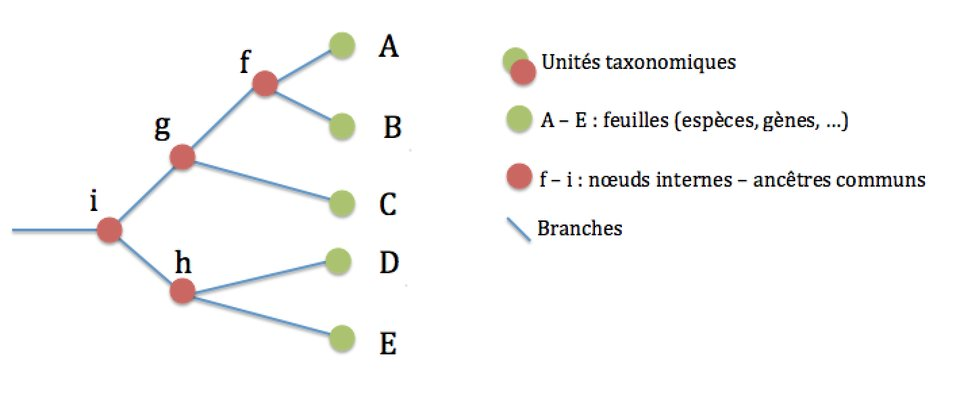
\includegraphics{Images/arbre_intro.jpg}
\caption{Arbre phylogénétique}
\end{figure}

\hspace*{0.5cm}

On observe des branchements successifs qui composent l'arbre
phylogénétique et à partir de ces données quantitatives observées, on
veut estimer la fonction de densité \(f\) qui donne la probabilité qu'un
nouveau branchement évolutif apparaisse après un certain temps.

Formellement, on a un échantillon \(X\)=\{\(X_1,\dots,X_n\)\} de
variables observées qui ont pour une fonction de densité
\(f \in \mathcal F\) où \(\mathcal F\) est un espace fonctionnel. On
cherche à estimer cette fontion densité \(f\) sur la quelle on fait le
moins d'hypothèses possible. On fera seulement les hypothèses
d'existance, de continuité et de positivité de la fonction \(f\).

D'où le choix du modèle suivant \(\{P=P_f,~f\in \mathcal F\}\) qui
revient à faire une estimation non-paramétrique de la densité. Ce qui
nous mène à la problématique de notre sujet.

\paragraph{Problématique}

Comment estimer la loi de densité de la création d'une nouvelle espèce
avec une méthode d'estimation non-paramétrique ?

Pour répondre à la problématque on cherchera à comprendre et finalement
implémenter un estimateur à noyau adaptatif, de type
Goldenshluger-Lepski sur des données d'arbres phylogénétiques.

\newpage

\section{Méthodes non-paramétriques}

\fancyhead[R]{Méthodes non-paramétriques}

\hspace*{0.5cm} En statistique, on parle d'estimation quand on cherche à
trouver certains paramètres inconus caractérisant une distribution à
partir d'un échantillon de données observées en se basant sur
différentes méthodes. On se tourne vers l'estimation non-paramétrique
lorsqu'on traite des paramètres à dimension infini. Ce qui est bien
notre cas, comme on cherche à estimer une fonction densité qui
appartient à un espace fonctionnel.\\
\hspace*{0.5cm} On présente dans la suite une courte introduction à
l'estimation non paramétrique. On introduira ensuite les deux classes
principales de l'estimation fonctionnelle (l'estimation par projection
et l'estimation à noyau) afin de discuter de ces deux classes et
expliquer pourquoi on fait le choix de l'estimation à noyau.

\subsection{Définitions}

\begin{definition}
    **Estimation non-paramétrique :**\newline
 L'estimation non-paramétrique vise à résoudre des problèmes d'estmation dans le cadre statistique où le modèle auquel on s'intéresse n'est pas décrit par un nombre fini de paramètres et dont chacun de ces paramètres ne permet pas de décrire la structure générale de la distribution des variables aléatoires.\newline Cela signifie qu'on utilise des modèles statistiques à dimension infini.
\end{definition}

Dans le cadre de notre problématique on s'intéresse a l'estimation de
densité.\newline Un des principes de base de l'estimation de la densité
selon une méthode d'estimation non-paramétrique est le suivant \newline

\begin{definition}
Pour un échantillon d'observations quantitatives $X=\{X_1, \dots,X_n\}$ de variables aléatoires i.i.d admettant une densité $f= F'$. Supposons que $f \in \mathcal F$ où $\mathcal{F}$ est un espace fonctionnel. On cherche à estimer la fonction de densité inconnue $f$ à partir de ces observations.\newline
On notera $\hat f_n$ l'estimateur de f.\newline
On se trouve donc avec le modèle suivant $\{\mathbb P=\mathbb P_f,~f \in \mathcal F\}$, 
tel que $\mathbb P_f$ est la mesure probabilté de la densité $f$.
\end{definition}

L'estimation ici concerne donc la fonction elle même plutôt que les
paramètres, ce qui explique le nom d'estimation
non-paramétrique.\newline

\begin{remark}  
- On notera dans la suite $\hat f$ l'estimateur de la vraie fonction $f$.  
- On considerera souvent les distances $L^p$ avec $p = 1,2$ ou $\infty$ .
\end{remark}

Une des premières estimations non-paramétriques de la fonction de
densité qui est possible est l'histogramme.

(ajout formule graphique)

L'histogramme fait partie de la famille des estimations à noyau qu'on
détaillera plus tard.

Il existe deux grandes familles de méthodes pour estimer une fonction
densité:\newline \hspace*{0.5cm} - L'estimation par projection et
\hspace*{0.5cm} - L'estimation par noyau.

\subsection{Estimateurs par projection :}

\begin{definition}
**Estimation par projection :** \newline
Supposant que la fonction $f$ à estimer est dans l'espace de Hilbert
$\mathcal F = (L^2 , \parallel\,.\parallel, <\,.,~.>_)$ avec $(\Phi_j)_{j>0}$ une base orthonormée de $L^2$, $\mathbb E _N$  un sous-espace fini de $\mathcal F$ et $1 \leq |N| < \infty$.\newline
De plus $a_{\lambda} = <f,\Phi_{\lambda}> = \int_{\mathbb R}f(x)\Phi_{\lambda}(x) dx$.\newline
Alors, on estime la fonction $f$ par son projeté 

$$
\Pi_N~f = \sum_{\lambda \in N} a_{\lambda} \Phi_{\lambda}
$$
\end{definition}

\begin{remark}
-Cette méthode nous ramène au cas paramétrique.\newline
\end{remark}

Dans la suite on procèdera à la méthode la plus fréquemment utilisée
pour l'estimation d'une densité : L'estimation à noyau.\newline 

(Argument pour le choix de la méthode à voir)

\subsection{Estimateur de densité à noyau :}

\fancyhead[R]{Estimateur de densité à noyau :}

\subsection{Evaluer un estimateur}

Avant de commencer cette partie on va d'abord introduire quelques
notions et définitions\newline

\begin{definition} {Noyau}  
On note par le noyau la fonction intégrable K$\mathbb{R}\rightarrow\mathbb{R}$ tel que:
$$\int_{\mathbb{R}}K(u)du =1$$
et soient $h<0$ le paramètre de lissage.\newline $K_h : u\in \mathbb{R} \rightarrow K(\frac{u}{h})/h$

\end{definition}

\begin{lemma}
On peut approximer la famille $(K_h)_{h>0}$ par l'identité du produit de convolution.
\end{lemma}

\begin{demonstration}
A Faire
\end{demonstration}

\begin{corollary}
$K_h * f : x \rightarrow \int_{\mathbb R} K_h(y-x) f(x) dx$ tend vers la fonction f quand h tend vers 0.(pour la distance $L^2$)
\end{corollary}

Pour évaluer un estimateur on définit le risque associé d'un estimateur
\(\hat f\) pour l'estimateur f.\newline **Pas comppris**

\begin{definition} 
La fonction de risque : 
$$ 
\mathcal R(\hat f ,f)=\mathbb E_f[\parallel\hat f -f\parallel^2]
$$
\end{definition}

\begin{remark}
  La fonction de risque associé nous permet de comparer l'estimateur $\hat f$ et l'estimation f.\newline
On cherche à ce que ce risque associé soit minimal (i.e tend vers 0 pour un nombre d'observation assez grand).\newline
\end{remark}

\subsubsection{Risque quadratique ponctuel des estimateurs à noyau sur les classe des espaces de Hölder}

Nous nous intéressons au risque quadratique ponctuel de \(\hat{f}_n\),
i.e étant donné\newline \(x_0 \in \mathbb{R}\)

\[
R(\hat {f}_n, f) = \mathbb{E}[|\hat {f}_n(x_0) - f(x_0)|^2]
\]

Rappelons la décomposition ``biais au carré + variance'' du risque
quadratique:

\[
  \mathbb{E}[|\hat {f}_n(x_0) - f(x_0)|^2] = (\mathbb{E}[\hat {f}_n(x_0)] - f(x_0))^2 + \mathbb{V}(\hat {f}_n(x_0))
\]

\paragraph{Majoration du biais et de la variance}

Dans cette section, nous allons nous intérresser au compromis
biais-variance afin de minimiser le risque quadatique. Les duex
propositions suivantes montrent que sous certaines hypothèses, on peut
majorer le biais ainsi que la variance.\newline

\begin{definition} : Soit $l \in \mathbb{N^*}$. On dit que le noyau $K$ est d'ordre $l$ si $u^jK(u)$ est intégrable et $\int u^jK(u)du = 0$, $j = {1,...,l}$.\newline
\end{definition}

\begin{proposition}: Si $f \in \sum(\beta,L)$ avec $\beta > 0$ et $L > 0$ et si $K$ est un noyau d'ordre $l = \left\lfloor{\beta}\right\rfloor$ tel que $\int |{u}^{\beta}|\,.|{K(u)}|~du < \infty$ alors pour tout $x_0 \in \mathbb{R}$, et pour tout $h>0$ le biais peut être borné comme suit:

$$
|\mathbb{E}[\hat{f}_n(x_0)] - f(x_0)|\leqslant \frac{h^{\beta}L}{l!}\int|u|^{\beta}|K(u)|du
$$
\end{proposition}

\begin{demonstration}: (voir Esti-non para.pdf page 97, prop 4.10).\newline

   Le biais au carré tend vers zéro à la vitesse $h^{2\beta}$. Plus la fonction $f$ est régulière, plus le biais tend vite vers zéro quand $h$ tend vers zéro (à condition bien sûr que l'ordre du noyau soit suffisamment grand).\newline
\end{demonstration} 
\begin{proposition}: Si $f$ est bornée et si $K$ est de carré intégrable alors 

$$
\mathbb{V}(\hat {f}_n(x_0)) \leqslant \frac{\begin{Vmatrix}f\end{Vmatrix}_{\infty}\begin{Vmatrix}K\end{Vmatrix}^2_2}{nh}
$$

En particulier, si $f \in \sum(\beta,L)$ alors
$$
\mathbb{V}(\hat{f}_n(x_0))\leqslant\frac{M(\beta, L)}{nh}
$$
\end{proposition}
\begin{demonstration}:


$$
\begin{aligned}
\mathbb{V}(\hat {f}_n(x_0)) &= \mathbb{V}(\frac{1}{nh}\sum_{i=1}^nK(\frac{X_i-x_0}{h})) \\
&=\sum_{i=1}^n\mathbb{V}(\frac{1}{nh}K(\frac{X_i-x_0}{h})) \\
&=\sum_{i=1}^n\mathbb{V}(\frac{1}{nh}K(\frac{X_i-x_0}{h}))  \\           &=\sum_{i=1}^n\frac{1}{n^2h^2}\mathbb{V}(K(\frac{X_i-x_0}{h})) \\
&=\frac{1}{nh^2}\mathbb{V}(K(\frac{X_1-x_0}{h}) \\
&\leqslant \frac{1}{nh^2}\mathbb{E}(K^2(\frac{X_1-x_0}{h})) \\
&=\frac{1}{nh^2}\int K^2(\frac{u-x_0}{h}f(u)du \\
&=\frac{1}{nh}\int K^2(v)f(x_0 +vh)dv
\end{aligned}
$$ 


Et enfin,on admet le résultat suivant : \newline
il existe une constante positive $M(\beta,L)$ tel que $\begin{Vmatrix}f\end{Vmatrix}_{\infty} \leqslant M(\beta, L)$. Ceci implique que :

$$
 \mathbb{V}(\hat {f}_n(x_0))\leqslant\frac{1}{nh}M(\beta, L)\int K^2(v)dv 
$$ 
 \end{demonstration}

Pour que la variance tende vers zéro, il faut que \(nh\) tende vers
l'infini. En particulier, à \(n\) fixé, la variance est une fonction
décroissante de \(h\). Il y a donc une valeur optimale de \(h\) qui doit
réaliser l'équilibre entre le biais au carrré et la variance. On peut à
présent donner un contrôle du risque quadratique par le théorême
suivant.

\begin{theorem} Soit $\beta>0$ et $L>0$ et $K$ un noyau de carré intégrable et d'ordre $\left\lfloor{\beta}\right\rfloor$ tel que $\int |u^{\beta}|\,.|K(u)|du<\infty$. Alors, en choissant une fenêtre de la forme $h=cn^{-\frac{1}{2\beta+1}}$ avec une constante $c>0$, on obtient pour tout $x_0 \in \mathbb{R}$,

$$ 
R(\hat {f}_n(x_0)),\sum_d(\beta, L)):= \underset{f\in\sum_d(\beta,L)}{sup}\mathbb{E}[|\hat {f}_n(x_0)-f(x_0)|^2]\leqslant Cn^{-\frac{2\beta}{2\beta+1}}
$$ 
 où $C$ est une constante dépendant de $L,\  \beta, \ c$ et $K$.
 \end{theorem}
\begin{demonstration}: 
  On a

$$
 R(\hat {f}_n(x_0),f(x_0))= \text{Biais + Variance}
$$ 

   Si nous nous référons aux deux propositions précédentes, nous pouvons écrire :

$$
 R(\hat {f}_n(x_0),f(x_0))\leqslant(\frac{h^{\beta}L}{l!}\int |u|^{\beta}|K(u)|du)^2 + \frac{M(\beta,L)\begin{Vmatrix}K\end{Vmatrix}_2^2}{nh}
$$

On cherche ensuite la fenêtre $h$ qui minimise cette quantité. Comme on ne se soucie pas vraiment des constantes exactes quand on cherche la vitesse de convergence d'un estimateur, on utilisera la notation $c_1=(\frac{L}{l!}\int |u|^{\beta}|K(u)|du)^2$ et $c_2=\frac{M(\beta,L)\begin{Vmatrix}K\end{Vmatrix}_2^2}{nh}$. On doit alors minimiser en $h$ la quantité :


$$
  c_1h^{2\beta}+\frac{c_2}{nh}
$$

On a une quantité croissante et une quantité décroissante en $h$. Encore une fois, comme on ne se soucie pas pas des constantes, donc on cherche la fenêtre $h$ qui nous donne l'ordre minimal du risque. Quand $h$ est trop grand, le biais est trop grand, et quand $h$ est trop petit, c'est la variance qui est trop grande. On cherche donc la fenêtre $h$ qui réalise un équilibre entre le biais au carré et la variance:

$$ 
  h^{2\beta}\approx\frac{1}{nh}
$$
où le signe $\approx$ signifie ici "de l'ordre de". Cela donne :

$$
  h\approx n^{-\frac{1}{2\beta +1}}
$$

Autrement dit, pour une fenêtre $h$ de l'odre de $n^{-\frac{1}{2\beta+1}}$, le biais au carré et la variance sont de même ordre.Plus exactement, on choisit la fenêtre $h_*=cn^{-\frac{1}{2\beta+1}}$, avec $c$ une constante positive, on a :

$$
  Biais\ au\ carré \approx h_{*}^{2\beta}\approx Variance\approx \frac{1}{nh_{*}}
$$

De plus, on a alors :
$$
  h_* \approx n^{-\frac{2\beta}{2\beta + 1}}
$$

 
Autrement dit, il existe une certaine constante $C$ telle que, pour cette fenêtre $h_*$, on a :

$$
  R(\hat {f}_n(x_0),\sum_d(\beta,L))\leqslant Cn^{\frac{-2\beta}{2\beta + 1}}
$$

  Cette fenêtre est donc optimale à une constante près (si on change $c$, on change $C$ ça ne change pas le taux qui est $n^{\frac{-2\beta}{2\beta+1}}$).\newline
\end{demonstration}
\begin{remark}:  
  * L'estimatimateur dépend de $\beta$ à travers la fenêtre $h$. Or, sans   connaissance a priori sur les propriétés de la fonction $f$, on ne peut donc pas utiliser cet estimateur. On essaie alors de trouver un choix de fenêtre ne dépendant que des données et qui soit aussi performant (ou presque) que l'estimateur utilisant cette fenêtre optimale. A ce sujet, on introduira plus loin un choix de fenêtr ne dépendant que des données et qui est basé sur ce qu'on appelle la validation croisée (ou "cross validation" en Anglais).  
  * Nous avons vu plus haut que le biais au carré tend vers zéro quand $h$ tend vers zéro (si $\beta$ est suffisamment grand). Nous en déduisons la convergence de l'espérance de l'estimateur à noyau $\hat {f}_n$ vers la fonction $f$. Et donc, l'estimateur à noyau est asymptotiquement sans biais, $\hat {f}_n$ est consistante.\newline
\end{remark}

\begin{proposition}

Dans le cas d'un estimateur à noyau, on a :\newline
$$
R(\hat{f},f)=\mathbb E_f[\parallel\hat{f}-f\parallel^2 ] = \parallel f-K_h*f \parallel^2 + \mathbb E_f[\parallel\hat{f}-K_h*f \parallel^2]
$$
\end{proposition}

\begin{demonstration}
On que :\newline 


$\mathbb E_f\parallel\hat{f}-f \parallel^2 = \mathbb {E}_f[\parallel\hat{f}+\mathbb {E}_f(\hat{f} )-(\mathbb {E}_f(\hat{f} )-f)\parallel ]^2$.\newline

$\mathbb E_f[\parallel\hat{f}-f \parallel]^2 = \mathbb {E}_f[\parallel\hat{f}+\mathbb E_f(\hat{f} )\parallel]^2 +\mathbb {E}_f[\parallel\mathbb {E}_f(\hat{f} )-f\parallel] ^2 - 2~\mathbb {E}_f[<\hat{f}-\mathbb {E}_f(\hat{f});\mathbb {E}_f(\hat{f})-f>]$.\newline

Comme $\hat{f}$ est déterministe\newline 
$2~\mathbb {E}_f(<\hat{f}-\mathbb E_f(\hat{f})~;~\mathbb {E}_f(\hat{f})-f>)=2<0,~\mathbb E_f(\hat{f})-f>=0$\newline
Ainsi $\parallel\mathbb {E}_f(\hat{f} )-f\parallel$ est déterministe\newline
On obtient :\newline
$R(\hat{f},f)=\mathbb {E}_f[\parallel\hat{f}-f\parallel^2 ] = \parallel f-K_h*f \parallel^2 + \mathbb {E}_f[\parallel\hat{f}-K_h*f\parallel^2]$ 
\end{demonstration}

On a bien trouvé que : \[R(\hat{f},f)=biais^2+\mathbb Var\]

\begin{remark}\
   Plus la  valeur de h est grande, plus le biais devient grand et la variance petite et de même ;  
   plus la valeur de h est petite plus le biais devient petit et la variance explose.\newline
\end{remark}

Donc, afin de minimiser l'expression du risque le choix de h est très
influent et même plus crucial pour la qualité de l'estimateur que celui
de la noyau \(K\).\newline On doit chercher le meilleur compromis
biais-variance pour avoir un risque minimal.\newline Un paramètre trop
faible provoque l'apparition de détails artificiels sur le graph de
l'estimateur (La variance devient trop grande), par contre si on prend
une valeur de h très grande on aura la majorité des caractéristiques
effacées.\newline

\hspace*{4cm}
\href{http://chimix.com/an16/pol16/image/aspts35.jpg}{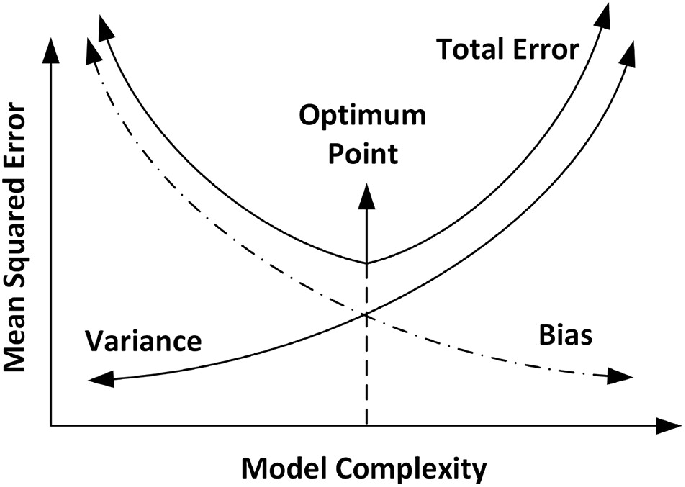
\includegraphics[width=3.22917in,height=\textheight]{Images/Bias-variance-trade-off.jpg}}

\subsection{Méthodes adaptatives :}

\hspace*{0.5cm} On a introduit précédemment la notion de l'estimation de
la densité qui dépend d'un paramètre de lissage h. Soit
\((\hat{f_h})_{h\in \mathcal H}\) une famille des estimateurs de la vrai
fonction densité \(f\) .\newline La question qui se pose est donc la
suivante : comment peut on construire un estimateur à risque optimal à
partir de cette famille (en prenant en considération les observations) ?
\newline \hspace*{0.5cm} Dans cette partie et afin de repondre a la
question qu'on a poser on va discuter au premier temps du choix du
noyau. Ensuite, on va introduir deux méthodes pour le choix du paramètre
de lissage h .

\subsubsection{Choix du noyau}

\subsubsection{Choix de la fenêtre}

L'estimation de densité nécessite le choix de la fentêtre qu'on note
h.\newline En statistique non-paramétrique, ils éxistent plusieurs
méthodes et critéres de qualité pour le choix de la fêntere.\newline

On présente dans la suite deux méthodes:\newline \hspace*{0.5cm} Méthode
de validation croisée.\newline \hspace*{0.5cm} Méthode de
Goldenshluger-Lepski.\newline

\paragraph{Choix de la fenêtre $h$ par validation croisée}

Le choix de la fenêtre dans la section précédnte est criticable: comme
on l'a mentionné, il dépend de la régularité la fonction \(f\) qui est
inconnue dans notre cas. On peut donc essayer d'estimer cette fenêtre
idéale par un estimateur \(\hat {h}\). De façon à souligner la
dépendance à la fonction, on va noter \(\hat {f}_{n,h}\) l'estimateur
associé à un choix de fenêtre \(h\). L'estimateur final sera
\(\hat{f}_{n,\hat{h}}\), une fois le choix de \(\hat{h}\) fait.\newline
On c herche à minimiser en \(h\) la le risque quadratique pour la
distance \(L_2\):

\[
\begin{aligned}
R(\hat {f}_{n,h})&=\mathbb{E}[\begin{Vmatrix}\hat {f}_{n,h}-f\end{Vmatrix}_2^2]\\        
&= \mathbb{E}[\begin{Vmatrix}\hat {f}_{n,h}\end{Vmatrix}_2^2] -2~\mathbb{E}[\int \hat {f}_{n,h}(x)f(x)dx] +\begin{Vmatrix}f\end{Vmatrix}_2^2
\end{aligned}
\]

Or la fonction \(f\) étant inconnue, ce risque n'est pas calculable à
partir des données. On cherche donc à estimer ce risque en utilisant
uniquement les données. Remarquons tout de suite que minimiser en \(h\)
la quantité \(R(\hat {f}_{n,h}, f)\) est équivalent à minimiser en \(h\)
la quantité \(R(\hat {f}_{n,h}, f)-\begin{Vmatrix}f\end{Vmatrix}_2^2\).
On va en fait remplacer la minimisation de la quantité inconnue
\(R(\hat {f}_{n,h}, f)-\begin{Vmatrix}f\end{Vmatrix}_2^2\) par la
minimisation d'un estimateur \(\hat {R}(h)\) de cette quantité. Plus
précisément on va chercher un estimateur sans biais de cette expression:

\[
\mathbb{E}[\begin{Vmatrix}\hat {f}_{n,h}\end{Vmatrix}_2^2] -2~\mathbb{E}[\int \hat {f}_{n,h}(x)f(x)dx]
\]

Le premier terme admet
\(\begin{Vmatrix}\hat {f}_{n,h}\end{Vmatrix}_2^2\) comme estimateur
trivial (d'après la propriété des estimateurs sans biais:
\(\mathbb{E}[\hat {\beta}]=\beta)\).\newline Il reste à trouver un
estimateur sans biais du second terme. Pour cela, nous admettons par
construction l'estimateur sans biais \(\hat {G}\) défini en tout points
sauf en \(X_i\) (c'est le principe du Leave-one-out):

\[
\hat{G} = \frac{1}{n}\sum_{i=1}^n\hat {f}_{n,h}^{(-i)}(X_i)
\] avec

\[
  \hat {f}_{n,h}^{(-i)}(x)= \frac{1}{n-1}\frac{1}{h}\sum_{j=1,j\ne i}^nK(\frac{x-X_j}{h})
\]

Montrons que
\(\mathbb{E}(\hat{G})=\mathbb{E}[\int \hat{f}_{n,h}(x)f(x)dx]\).\newline
Comme les \(X_i\) sont i.i.d., d'une part nous avons \[
\begin{aligned}
\mathbb{E}[\int \hat {f}_{n,h}(x)f(x)dx]&= \mathbb{E}[\int \frac {1}{nh}\sum_{i=1}^nK(\frac {x-X_i}{h})f(x)dx]\\
&=\frac{1}{h}\mathbb{E}[\int K(\frac {x-x_1}{h})f(x)dx] \\
&=\frac{1}{h}\int f(x)\int K(\frac {x-X_1}{h})f(x_1)dx_1dx
\end{aligned}
\]

D'autre part, nous avons \[ 
\begin{aligned}
\mathbb{E}[\hat{G}]&=\mathbb{E}[\frac{1}{n}\sum_{i=1}^n\hat{f}_{n,h}^{(-i)}(X_i)]\\
&=\mathbb{E}[\hat{f}_{n,h}^{(-1)}(X_1)]\\
&=\mathbb{E}[\frac{1}{n(n-1)h}\sum_{j\ne 1}K(\frac{X_j-X_1}{h})]\\
&=\mathbb{E}[\frac{1}{h}K(\frac{X-X_1}{h})]\\
&=\frac{1}{h}\int f(x)\int K(\frac{x-x_1}{h})f(x_1)dx_1dx\\
&=\mathbb{E}[\int \hat{f}_{n,h}(x)f(x)dx] 
\end{aligned}
\]

Donc, \(\hat{G}\) est un estimateur sans biais de
\(\int\hat{f}_{n,h}(x)f(x)dx\). Finalement, l'estimateur sans biais de
\(R(\hat{f}_{n,h}, f)-\begin{Vmatrix}{f}\end{Vmatrix}_2^2\) est donné
par:

\[
\hat{R}(h)=\begin{Vmatrix}\hat{f}_{n,h}\end{Vmatrix}_2^2-\frac{2}{n(n-1)}\sum_{i=1}\sum_{j=1,j\ne i}\frac{1}{h}K(\frac{X_i-X_j}{h})
\]

On définit alors

\[
\hat{h} = arg\ \underset{h\in H}{min}\hat{R}(h)
\]

Si ce minimum est atteint. On cherche une fenêtre parmi une grille finie
de valeurs, grille qu'on a notée \(H\) dans la formule ci-dessus.\\
L'estimateur \(\hat{f}_{n,\hat{h}}\) a de bonnes propriétés pratiques et
de consistence. La validation croisée est une méthode très générale mais
nous l'utilisons ici pour le choix la fenêtre \(h\) optimale.

\paragraph{Méthode de  Goldenshluger-Lepski}

La méthode de Lepski donne principalement des critères pour le choix
entre estimateurs à noyau \((\hat{f_h})_{h\in \mathcal H}\) avec
différentes fenêtres qu'on fixe en prennant n considération
l'échantillon des observations.\newline Cette méthode propose de choisir
le \(\hat h\) qui minimise l'expression suivante: \[
B(h)+V(h)
\] Avec :

\[
B(h)=sup_{h' \in \mathcal H}{[\parallel\hat f_{h'} - \hat f _h \parallel-V(h')]}
\] Et \[
V(h)=a \frac{\parallelK_{h'}\parallel^2}{n}
\] Tel que \(K\) est le noyau, \(a\) un paramètre et \(V(h)\) est le
terme de pénalisation.\newline

On a donc le \(\hat h\) est égale à: \[
\hat h = arg min_{h \in \mathcal H}(B(h)+V(h))
\]

\begin{remark}
Le terme de pénalisation choisi est proportionnel à la variance de l'estimateur.
\end{remark}

On s'intéresse dans cette méthode à déterminer le terme de pénalisation
minimal \(V(h)\) tel que si on le dépasse on n'obtient plus l'équilibre
biais-variance.\newline

Dans ce cas, la valeur de \(\hat h\) est d'ordre \(\frac{1}{n}\),

Le choix optimal de la fenétre h suivant cette méthode dans ce cas est
\(n^{-\frac{1}{2 \alpha +1}}\)

\end{document}
